\documentclass{article}
\usepackage[utf8]{inputenc}
\usepackage[natbibapa]{apacite} % citations
\usepackage[onehalfspacing]{setspace} % double spacing
\usepackage[dvipsnames]{xcolor}
\usepackage{cancel}
\usepackage[english]{babel}
\usepackage{graphicx}
\usepackage{placeins}
\usepackage{url,hyperref, lineno, microtype,subcaption}
\usepackage{tikz}
\usepackage{csquotes}

% revision color
\newcommand{\rev}[1]{{\color{ForestGreen}#1}}

% commenting/notes color
\newcommand{\comment}[1]{{\color{red}#1}}

% checkmark
\def\checkmark{{\color{ForestGreen} \tikz\fill[scale=0.6](0,.35) -- (.25,0) -- (1,.7) -- (.25,.15) -- cycle;}} 

\citestyle{apacite}
\bibliographystyle{apacite}

\newlength{\cslhangindent}
\setlength{\cslhangindent}{1.5em}
\newenvironment{cslreferences}%
  {}%
  {\par}
\begin{document}
\begin{center}
{\Large\bf Author response to reviews of Manuscript \textcolor{blue}{abn9889}}
\end{center}
{\Large Foraging complexity and the evolution of childhood.}\\[1em]
{Ilaria Pretelli, Erik Ringen, Sheina Lew-Levy}\\

We thank the three reviewers for detailed and considered feedback. By responding to their feedback, we feel that we have strengthened the clarity and theoretical importance of our paper. Specifically, we have expanded the introduction and discussion, and clarified the methods in the text and in the supplementary materials. Below we \rev{respond to each comment in green}.

\section{Reviewer 1}
This paper is well written and provides an important contribution. It was a delight to review. That being said, I recommend a re-frame below. Not a reanalysis of data, but a change to how the paper is set up so that the body of the paper (and the resultant conclusions) are an accurate reflection of what the study aimed to do –test the embodied capital hypothesis using a robust data set. The notion that childhood co-evolved with complex foraging is supported by these data – but not novel to this paper and not introduced for the first time here.
The beautiful and compelling analyses of published cross-cultural data, the different proficiency schedules, and the first large-scale analysis of resources by complexity of collection are new – and a very welcome contribution to the literature. It is for this reason that I recommend a revise and resubmit.


\rev{We thank the reviewer for the positive comments. We also took seriously the request for a clearer introduction to the hypotheses offered for the evolution of childhood, as I describe below. }

\subsection{General Comments:}
\begin{enumerate}
    \item The introduction is well-written – but introduces the issue at hand without a thorough treatment of life history theory. This is a weakness of the paper in its current form. Many young scholars just learning about life history theory erroneously conclude that life history theory is equivalent to embodied capital theory. Many introductory textbooks in our discipline do not offer any alternative explanatory models to delayed development other than embodied capital – it is often taught as the ONLY model of why childhood evolved. Thus, the authors have an opportunity and a responsibility in this paper and in this high profile outlet to introduce the opposing theoretical paradigms and to articulate that they are, in fact, testing one of these.

\rev{We have now incorporated this feedback throughout the entirety of the introduction. Specifically, we now succinctly outline the key approach of life history theory and outline the two major competing hypotheses regarding the evolution of childhood. We then state key Embodied Capital Theory predictions, and outline supporting and opposing studies which tested these predictions. Please see new sections of the introduction (in red in the text). }

    \item Specifically, Kaplan’s embodied capital hypothesis is introduced early on without any citations highlighting other evolutionary models (e.g. Charnov, etc). I am not necessarily suggesting that the authors set up the article as a test between the two models, but it should be set up as a test of the embodied capital hypothesis, as that is what it is. For example, Bird and Bliege Bird’s work [citation 11] on size and strength is introduced in a long generic list on studies of foraging proficiency. The fact that alternative evolutionary models have been proposed for the evolution of childhood and the development of complex foraging tasks should not be ignored – it needs to be stated up front. Once that has been established, then the argumentation can proceed as written. See detailed comment on Charnovian life history below. Also, note specific comment \#6 below. If children reach adult levels of production for fruit and fish/shellfish early in life, whereas production for tubers and game continue into adulthood – this may be interpreted by many as support for Charnovian models (as Bird and Bliege Bird have found with Martu). This interpretation of the data as supporting ECT (which is the notion that childhood evolved with complex foraging skills) needs to be clearly argued.

\rev{In addition to the changes made throughout the introduction (see point 1) we have addressed this more explicitly in relation to skill in the discussion as follows (PX): 
%Our novel analysis allowed us to explicitly estimate skill. This measure likely reflects various individual traits that contribute to skill, including somatic and cognitive traits such as strength to knowledge. An implication of ECT is that cognitive more than somatic traits are the limiting factor when foraging complex resources. In their research with Mardu and Meriam, Bliege Bird and Bird \citep{bird_constraints_2002, bird_mardu_2005} find that foraging performances are largely constraint by size. However, knowledge was not explicitly measured in their analyses. Considering that size, strength, and knowledge tend to develop together \citep{bock_what_2005}, it remains unclear whether their findings are at odds with, or complementary to, predictions derived from ECT. Similarly, and because few studies consistently report individual measures for size, strength, and knowledge, our measure for skill does not differentiate between different types of embodied capital. Instead, our findings suggest that in order to target complex resources, children require high levels of skill, which they acquire through an unknown combination of learning and growing. Nonetheless, the difference observed across resource complexity is consistent with the coevolution between early life history traits and the especially complex niche targeted by our species. We look forward to future studies which collect data on various aspects of embodied capital in order to tease apart their relative contribution to foraging skill across resource types. 
}

    \item What type of game needs to be stated up front. Small/medium game are not the same as large game. If all animal protein was treated in the same way (lumped together), this needs to be stated and then listed as a limitation. See specific comment \#5 below.

\rev{Thanks for pointing this out. Indeed, this discrepancy is one we ourselves outline in the introduction (PX): 

%Still, children can achieve high returns by specializing in hunting matched to their size, skill, and strength. For example, Australian Martu children hunt goanna lizards in rocky outcrops, where they can maximize their returns given their height, stride length, and walking speed (10). 

Unfortunately, this discrepancy is not one which we can address using the available literature. This is because the majority of studies on hunting, including those in the \texttt{cchunts} package, do not report the type of prey or technique used. 

We now specifically state this in the methods (PX):
%Note that because it is rarely reported in the publish literature, we were not able to account for variation in game size, though we acknowledge that there may be substantial differences in skill development for small and large game.

We now more explicitly highlight that this is a crucial area for future research in the limitations at the end of the discussion (PX):
%Future studies should also consider heterogeneity in complexity within resource types across regions, seasons, and based on available extractive technologies. For example, while we considered hunting more generally, prey types vary by size, seasonal abundance, distribution, and the availability of efficient hunting technologies. Future studies should consider this variation when reporting on hunting returns.
}
\end{enumerate}

\subsection{Specific comments:}
\begin{enumerate}
    \item The Charnovian model must be introduced. In the current paper it is glossed over. The Martu data, for example, are directly in line with the argument (and the title of the authors’ own paper) that successful hunting is associated with constraints on growing – not knowing. In direct opposition to embodied capital. This paper should not be introduced without first introducing the alternative evolutionary model for which this study supports. See summary of Charnov and Charnov and Berrigan in Bird and Bird (2002). A direct quote from Bird and Bird, underscoring their orienting evolutionary model, is as follows: “experience and social learning in primates are important, beneficial consequences of juvenility but may not necessarily be the cause of delayed maturation.” Thus, citing this study without introducing the orienting evolutionary model, which stresses selection pressure on low adult mortality rates (not on experiential learning) needs to be rectified in the revision. First sentence in the Discussion is strong. This should be reworked in the beginning of the paper to reframe it: “Childhood is theorized to have evolved as an extended learning period for collecting complex resources. Yet, no studies to-date have explicitly modeled the association between resource complexity and children’s productivity.” That is the paper – and that is the contribution. First test of embodied capital by actually looking at resource complexity. Which is a substantial contribution to the literature and should be applauded. Another place ECT is explicitly supported: “Thus, while these species do collect complex resources, they do not specialize in them. Humans, on the other hand, preferentially target complex resources (8, 41).” Both supporting citations are authored by proponents of ECT and support that model.
    
\rev{We have now changed our opening paragraph as follows (PX):

%Human childhoods are characterized by slow physical growth, extended dependence on parents and alloparents for provisioning, and increased investment in brain growth compared to nonhuman primates (1–5). Multiple hypotheses derived from life history theory have aimed to explain how this constellation of features was selected to maximize lifetime fitness. Following Charnov’s dimensionless numbers model (6), which finds regular patterns of covariation between total life span and age at first birth across species, some researchers have suggested that human childhood is a by-product of our long total lifespans (7). Alternatively, the Embodied Capital Theory (ECT) posits that human childhood evolved alongside our increased reliance on the complex foraging niche typical for our species (8). Difficult-to-acquire, energy-packed resources compose a large proportion of human diets. The exploitation of these resources require high levels of coordination, strength, knowledge and/or other cognitive skills. ECT hypothesizes that these traits–collectively termed “embodied capital”–are acquired during a protracted development. Under the assumptions of ECT, the costs associated with low productivity in early life and high rates of parental provisioning are offset by high lifetime productivity.

We also now more explicitly state that our findings support predictions from ECT in the discussion (PX):
%These findings support the view that complex resources require a longer investment in learning, and thus, in line with ECT, may have promoted the evolution of childhood. 
}

    \item I applaud the cross-cultural data and the articulation that cross-cultural data are important to understanding variation and the proficiency schedules. That being said, the evolutionary model for why childhood evolved necessarily takes variation into account. Meaning, at the end of the paper, the authors argue (with beautiful attention paid to cross- cultural variation) that childhood, indeed, co-evolved with a complex foraging niche. Much more cultural and ecological context provided (badly needed! So thank you to the authors) – but remains a support of embodied capital and should be framed as such.

\rev{We now more explicitly make reference to the support of ECT in our concluding paragraph:
%In support of ECT, this finding is consistent with with the view that long childhoods evolved as an extended period to learn to exploit the most complex resources in our foraging niches.
}

    \item This is a powerful sentence:“Using these data, we quantify how skill-intensive different resources are and assess whether children’s proficiency increases more slowly for more skill-intensive resources.” This should be what the abstract focuses on – that, despite all of the work on children’sforaging (and the persistent battles between ECT and Charnovian models) for decades, quantified large-scale cross-cultural data on proficiency by resource remains undervalued and understudied. The authors rectify that here. The fact that these data support ECT is almost beside the point. But given that the authors set it up as an evolutionary investigation, it must necessarily introduce the debate. Then I suggest moving away from it and highlighting their excellent analyses and discussion.
\rev{Thank you for this comment. We have attempted to reframe the introduction to highlight this contribution (see response to general comment 1). We have also now highlighted this more explicitly in the abstract:
%abstract goes here
}

    \item Again, authors are dancing around the issue. Adeptly, but still dancing. “Our approach can thus help resolve outstanding contradictions regarding children’s foraging proficiency and skill ontogeny in the published literature.” What contradictions? Spell them out for the reader. This leaves a reader unfamiliar with the literature questioning what the authors are actually interrogating. Conclusion is: “This finding is consistent with the view that long childhoods evolved as an extended period to learn to exploit the most complex resources in our foraging niches.” This is in support of ECT. For some reason the authors seem resistant to naming that. It remains unclear why.


\rev{As noted, we have now made the theoretical links of our finding more explicit throughout. More specifically, we have outlined the discrepancies as follows (PX-X):
%Several lines of empirical research using data from contemporary subsistence societies have aimed to test one of ECT’s key predictions: that early life productivity should be low, with children’s foraging proficiency increasing with age alongside gains in knowledge, skill, and experience (9–16). Support for this prediction has been mixed. [...] These mixed findings may be resolved by considering another of ECT’s key predictions: that the difficulty of acquisition explains the age profile of production (8), with more difficult-to-acquire resources requiring longer investment in skill development. Yet few studies have explicitly tested this prediction. 
}

    \item Authors consistently use the term, “game”. They should differentiate between large game and small/medium game. The same types of arrows are not even used for small/ medium game and large game in many societies using bows and arrows. How were small game handled in this study? In “Results” section, should indicate size of game for these results. For example, Fig. S2 says “game” – is this all game? If so, this will have to be listed as a weakness of the paper. Skill targeting birds or riparian game, for instance, are very different levels compared to tracking large game animals that require poison tipped arrows to take down. Some small game is shown in the red figure, so it seems that “game” refers to all animal protein? Where is honey included? Is it ``mixed/other?”

\rev{In terms of 'game', we have now addressed this comment throughout the text. Please see our response to general comment 1}

    \item List out, somewhere in Supplemental (?), what these ``other” foods are. Why were the broad categories listed selected – to the exclusion of others? Expand in methods.
    
\rev{We include all available data in the estimation of general age specific trajectories, without biasing the main four categories of resources we are comparing. Eggs and honey, although often highly valued foods, are very rare in the available data on foraging and thus cannot be considered individually, and we did not have enough ethnographic understanding on how to integrate these two very different forms of foraging in one of the extant major categories. In the methods, we state this information as follows (PX):
If data points could not be attributed to specific resources, they were categorized as mixed, as were data relative to eggs and honey. These data contributed to the estimation of posterior values for the overall estimates, even if their data set-specific parameters are not presented in the resource comparisons.}

    \item The finding that young foragers reached adult levels of production for fruit and fish/shellfish early in life, yet the production for tubers and game continued into adulthood is key. Rather than as straightforward support for embodied capital, doesn’t this beg the question that these data might support Bird and Bliege Bird’s notion that it is size \& strength and not necessarily skill that are responsible here? If not, and the authors interpret these findings as support for ECT (which needs to be argued more clearly), then how this doesn’t match the Martu paper needs to be addressed. Martu kids reach shellfish proficiency earlier – just as shown here – but the orienting model is Charnovian (not ECT). That has to be addressed in the discussion. Also, a further limitation, the shellfish data are overwhelmingly from Bird and Bird (Fig. S6). Given the clear orienting model of the authors of those papers, it puts the responsibility firmly on the authors here to explain how their conclusion (similar to Bird and Bird) is in support of ECT and not a Charnovian model. Same data on shellfish, same conclusion (that with age, skill increases for only complex resources but not for easy to extract ones) – but different interpretation, it seems. 
\item \rev{Thanks for pointing this out. We now explicitly compare our findings to those of Bliege Bird and Bird in a new paragraph on skill in the discussion (see response to general comment 2). We have added the above-mentioned limitation as well (PX):
%Additionally, these study-specific parameters are highly correlated with resource type: with few exceptions, each study reports returns for only a single category of resource. This makes it difficult to confidently assess whether variation is due to true differences between resources or to unmeasured differences between populations or in study methodology. This issue is especially apparent for shellfish, where all the available data comes from the same research group. 
 }

    \item Fantastic sentence – very strong: “To better understand the resource-specific development of skill beyond the general estimation presented in the present paper, future studies should integrate ethnographic understanding of each population’s subsistence strategies, as well as individual-level measures of traits which may contribute to skill.”
    
\rev{We thank Reviewer 1!}
    
    \item The statistical model in R is impressive. These analyses represent what should be the gold standard, moving forward. Very well done.

\rev{Thanks again!}

\end{enumerate}

\section{Reviewer 2}
In their manuscript, “Foraging complexity and the evolution of childhood”, Pretelli et al.  assemble an exhaustive database of published sources on children's foraging to investigate how  foraging returns vary according to age and type of foraging activity. The main finding presented  is that age-trends are dictated most strongly by resource type, with the implication that long  childhoods would have evolved to facilitate increased focus on complex resources that take  longer to learn. Overall I find the paper to be excellent and I am very excited to see this  published. This is an exceptionally important topic which the authors address using great  attention to detail. The statistical modeling approach is commendable as it manages to make use  of a highly heterogeneous dataset that is comprised of a mix of data types (e.g., means/SE versus  individual returns), has outcomes on different scales, and includes many variables with  significant measurement error (age and even sex in cases where it wasn't properly differentiated  in the original studies).  I do, however, have several concerns with the manuscript that should be addressed during  revision. These concern primarily the interpretation of some results, comparability of data types,  and the novelty of the main conclusions (each described further below).
*Please note that line numbers are not included in the manuscript, so specifics are directed to the 
appropriate page

\rev{We thank Reviewer 2 for the positive comments and take seriously the concerns, as described below.}

\subsection{Major comments:}
\begin{enumerate}
    \item  I am surprised by some of the main interpretation of results. For example, the authors write "We found that, in general, foraging returns increase rapidly during early childhood and begin to plateau in adolescence (Figure 1a)." Looking at figure 1a, it appears that there is an extremely slight hint of faster exponential increase at the youngest lifestage (which has to exist because  newborn infants don't produce food, so there has to be a jump when any appreciable foraging starts) and otherwise the curve for the global average looks almost perfectly linear. My apologies if I am missing something obvious, but where exactly is there any hint of a plateau in adolescence? The authors go on to say that 72\% of productivity is achieved by age 10, and this is again repeated at the beginning of the discussion. Unless my eyes are really tricking me, that is not  what figure 1a shows. I apologize if this is my own failing in understanding, but perhaps other  readers would struggle as well if it is not clear to me? Figure S1, on the other hand, does seem to better show the described plateau for trends in skill. The captions suggest that Figure 1 is showing ``foraging returns" versus ``Skill" shown in figure S1, but the differences between these figures is hard to parse. The authors are clear at the end of  the intro that skill is modelled as a dimensionless latent variable and thus it is expected that plots of skill would not have y-axis units if skill is being shown here. But the figure 1 caption says ``foraging returns" and ``scaled by their maximum value", suggesting that there should be a y-axis here labeled something like \% of maximum value. Additional clarity is needed.
    
\rev{%Ilaria I'll let you work this out but I would just say something like: Thank you for catching this mistake. We have updated the text as follows (PX): 
%I also recommend you add the axes
We are a bit embarrassed to say that Reviewer 2 is completely correct in this assessment, and we did fail to update this part of the Results section as the rest of the draft changed. Indeed, the description opening the Results section is a refuse of a previous version in which we were describing in parallel the returns and skill results, currently presented in figure XXXX and XXXX. We updated the relevant passages in the main text and thank Reviewer 2 for having caught on this mistake. Reviewer 2 also points out that the absence of axes in the figures presenting the results could confuse the reader. We chose to leave the axes blank for exactly this reason, not to confuse the reader with overall meaningless units, as the values are on a relative scale. We could add axes as a visual guide, if the editor and/or Reviewer thinks it would be better to do so, but our preference would be for better explaining the unit free axes in the caption of the figures, as we did in the new draft.}

    \item On page 5 it notes that data were included if presented as continuous quantities such as  kcal/day or g/h. I wonder whether these units are actually comparable even when using well- justified statistical approach here. My concern is that one of these, g/h, represents a rate of  acquisition in which the denominator is time spent undertaking the specific foraging activity,  whereas the other, kcal/day, is also a rate of acquisition but one in which the denominator is time  independent of how much is spent on the specific foraging activity. As a result, the latter measure is heavily dependent on how much time foragers in a given society spend on each activity. So, there could be a situation where the same data in a society shows that foragers have a very high  rate of return (g/h) but have an extremely low daily return rate (kcal/day) simply because they  rarely do a given foraging activity but when they do it is highly profitable. Therefore, even relative age trends could be characterizing different phenomena as they might depend on more or less time devoted to a particular activity. Unfortunately, this could be a potentially serious flaw that doesn't seem to be remediated  by the latent variable approach (and incidentally makes it easier to overlook) if the measures are not comparable across studies.
    
\rev{This critique is definitely founded and we worried extensively about it. As Reviewer 2 points out, dealing with this problem with the current data is nearly impossible. We tried to take into account data collection methods in the analysis, with the idea, for example, that data collected as part of time allocation studies not focusing on foraging would be better representative of null returns and of actual return to time, while data recorded when foragers return to camp with prey would be biased towards successful trips, when the bounty could denounce to the researcher the goal of the trip. Unfortunately, on the one hand the methods reported in the papers do not always describe data collection strategies in detail, and on the other there seemed to be quite a lot of variation in these strategies, making it hard to group the studies and account for the differences appropriately. In answer to this comment, we highlight the implications of this problem in the limitations section of the Discussion.}

    \item The journal format in which methods are presented after results is unfortunate for this paper.  Because many of the outcome variables are non-intuitive model based quantities (e.g. skill and  elasticity of returns on skill), it does a disservice to readers to see results before the methods  because there is not enough information early in the paper for reasonable context. I understand  that the authors don't have control over this, but perhaps more methods material can be integrated earlier for those who won’t jump down before reading the results.
    
\rev{We extended the last paragraph of the Introduction section to provide a better explanation of the methods.}

    \item Finally, after reading I am left wondering how this analysis advances our understanding of  human life history evolution and whether more could be learned. As it stands, we are left with  the conclusion that "children's age-specific production varies with resource-specific skill intensity." In other words, the rate at which kids learn different foraging skills depends on how  difficult the foraging activity is. This is indeed a fair conclusion, but one that seems relatively  apparent from the literature cited by the authors. That said, I still see great value in compiling all this information into a synthesis and applying a  sophisticated model to draw general conclusions (so definitely not disparaging the work here).  But I do wonder whether there is any more that could be discussed in light of these findings. For  example, is there interesting variation across societies or due to habitat types that make hunting  or USO foraging more delayed and difficult-to-learn skills? Are there other society-level attributes such as age at first birth that affect population-level differences? Could the data  compiled here be leveraged in some way to actually address the central question raised about how capable children are of fully providing their own caloric needs, even if just from a subset of  populations? Lastly, the discussion has text calling for "researchers to consider these variables [ecological and social contexts] in their future research". Given that this paper is positioned as a  comprehensive synthesis on this topic, it is unfortunate that no attempt is made here to actually  delve into these interesting questions. These and a host of other tantalizing questions suggest that the analyses here don't go deep as they might beyond the relative age-curve shapes themselves.

\rev{It seems an excuse, but this answer starts again with 'there is not enough data'. Collecting foraging data requires huge amount of effort and much time, and most of it focuses on adult hunting. Focuses on these, the 2020 paper from Koster and colleagues does an amazing job of pulling together an impressive amount of individual level data. The tremendous amount of work (from contacting the authors to the organization of the data, so much effort must have gone into building this dataset--for which we are very grateful, as we draw from it) has been rewarded by a large, diverse, detailed dataset, although limited to hunting. When aiming to include other resources, and focusing on published sources, we knew we were going towards smaller, less precise datasets. This imposed severe limitations to our approach. For example, Reviewer 2 suggests here to look at geographic/environmental variation in USO, but our dataset comprises mainly data collected in Africa in arid or semi-arid conditions. Similarly, it would probably be a bit of a stretch to compare improvements in calorie collected, as returns are described as a combination of energetic content and weights, and many studies are not detailed enough to offer independent insight on temporal variation in the timing at which children become proficient foragers. More generally, though, we agree with Reviewer 2 on the fact that more could be said on geographic and environmental variation in the development of foraging skill. Many of the studies we analyzed offer interesting insight on how environment could be related to specific aspects of foraging. Many of these, though, are intuitive interpretations of patterns, rather than rigorous testing. In this paper we adopted a rigorous quantitative approach that not only brought us to exclude many studies that contain relevant insight, because of poor data quality, but also we tried to keep a simple framework of analysis, given the problems many of the datasets we included presented. Given the quality and diversity of the data, the inference we present in the paper are the only ones we feel we can confidently offer to a scientific audience. This said, future work \textit{should} pay attention to environmental variables and report them carefully, so that future researchers attempting to build on our efforts will have better quality data to work on. With the current set of available papers, we suggest that qualitative analysis would do a better job of describing and combining the intuitions of the many researchers that worked on this subject. } %CHECK WITH GUYS
\end{enumerate}

\subsection{Specific comments:}

\begin{enumerate}
    \item There are numerous typos throughout the references that should be fixed (for just one minor example, see (15) and the spelling of "Pum foragers". \rev{Thanks! This and others have been taken care of.}
    
    \item Intro, 1st paragraph: refs (6,7) are not the papers that should be credited with this original idea. It  would make much more sense to remove these and cite (8) there as well. \rev{Also opportunely modified.}
    
    \item Intro, 1st paragraph: where ref (8-10) is cited -- you should be certain not to miscite Hawkes (9)  here, given that the way it reads now would make it seem as though it endorses the embodied capital theory, which it most certainly does not. \rev{We believe that in our re-worked introduction the position of Prof. Hawkes is clearly defined in opposition of ECT. }
    
    \item ``Kaplan et al. (8) found that among Hiwi, Ache, and Hadza, individuals only produce more than they consume in mid-adulthood.": Why do the authors say "mid-adulthood"? The main figure  from that paper shows the composite hiwi/ache/hadza production curve becoming net positive  around age 18 or so (or would the authors say that 18 yrs old is mid-adulthood?). \rev{Text was appropriatedly changed to better reflect the different patterns among men (positive production at 18, ok a bit of a stretch to define it early adulthood) and women (who only become net producer around 45 years old, in the plot presented in the paper, probably because of increased consumption linked to reproduction). }
    
    \item  ``These have shown that for big game hunting, returns peak in mid-adulthood, several years after peak strength.": Should cite Koster et al. 2020 here. \rev{Definitely.}
    
    \item Page 2, 1st paragraph: There are more ethnographic examples that would be good to cite here. For example, Crittenden's 2016 book chapter (Chidren's foraging and play among the Hadza) has a nice description of the ontogeny of different animals kids hunt as they become increasingly  proficient. \rev{HERE}
    
    \item " a forager must know where to find plants carrying ripe fruit".: Is this true? Ethnographic  experience with hunter-gatherers would suggest that young individuals commonly carry out these activities in groups and at known collection locations that can be quickly/easily learned from other group members. \rev{This point has been specified in the introduction.}
    
    \item Fig 1 caption, " Dashed lines highlight major differentials across childhood": What does this mean? Is this referring to standard stages of development? Or differentials in shape of the fitted  curves? \rev{Dashed lines highlight arbitrary age differentials across childhood, and this has been specified in the caption.}
    
    \item What explains the long right-tailed distribution of elasticities of returns on skill? I'm struggling  to come up with an intuitive explanation, and wonder whether it has to do with variation across  societies? 
    
\rev{The long tails were a consequence of the log-link function for these parameters, e.g.,:  $elasticity = exp( a + a_sex + resource_v + outcome_v + sex_resource_v + sex_outcome_v )$ Even with regularizing priors on all of the individual additive components, once passed through the exponential function, there will be non-negligible prior probability on extreme, implausibly large values of eta. To remedy this, we have replaced the $exp(x)$ link with $log(1 + exp(x))$, which still gives the appropriate constraint on the range $(0,+Inf)$ but increases almost linearly as $x$ increases. See figure \ref{fig:reply_1}. With our new approach, those long tails have been pulled in. }

\begin{figure}
    \centering
    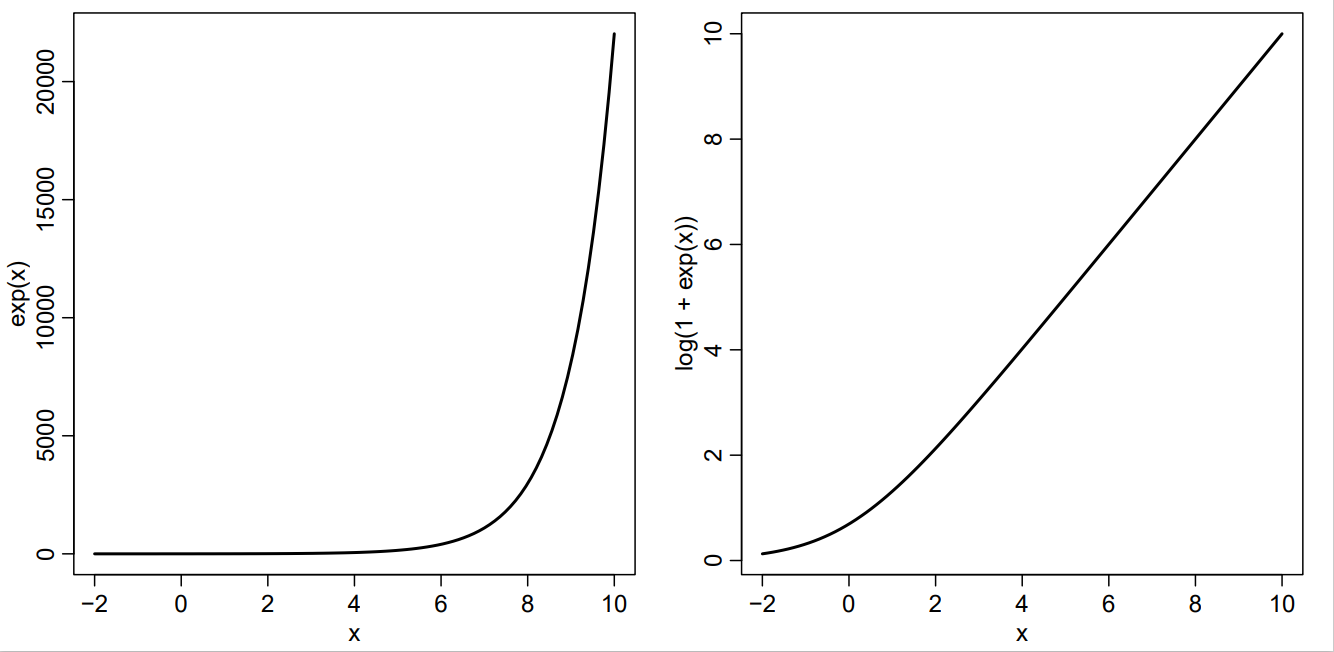
\includegraphics[width=12cm]{text/images/reply_1.png}
    \caption{Comparison between approaches that regularize values of eta.}
    \label{fig:reply_1}
\end{figure}
    
    \item ``This suggests that disparities in production between low skill and high skill foragers are more  apparent for more complex resource types." -- this statement is basically just saying that skill is  more important for resources that are more difficult to acquire. Seems kind of obvious, no? Also  the word ``complex" is ambiguous (later the authors use the words ``hard" and `easy") since that isn't really measured here (although one might rightfully argue that the elasticity of returns on skill is what best defines how complex a resource is). \rev{HERE}
    
    \item ``Yet, no studies to-date have explicitly modeled the association between resource complexity and children's productivity.": That is not entirely true -- other authors have described children's return rates across different resource types (similar to those investigated here), see e.g. Kramer,  Karen L. "Childhood Teaching and Learning among Savanna Pumé Hunter-Gatherers." Human  Nature 32.1 (2021): 87-114. The same goes for some other literature that the authors did cite. \rev{Some of the papers we include in our analysis do indeed compare qualitatively age-related changes in foraging, but a quantitative, precise comparison of foraging return rates by age for different resources has not been performed, to our knowledge. This said, we agree that the sentence could be debatable and slightly appropriately rephrased.}
    
    \item typo?: "hunt small preys" \rev{indeed}
    
    \item Discussion: The comparison of complexity of the human foraging niche with other primates is complicated given that elasticity of returns on skill hasn't (to my knowledge) been measured in  the same way in other primates. I see the point that other primates are focusing more on  resources that for humans show lower skill elasticities, but it is not clear elasticities behave  similarly across species (for example, does the fact that lions hunt mean that they have a  complex foraging niche? Do mole rats feeding on USOs have a complex foraging niche? Would  these foraging examples show high elasticity of returns for these species in the same way they do for humans?). \rev{Reviewer 2 makes a fair point, here. Mole rats enjoy a comparative advantage when feeding on USOs, compared to humans, because they are physically and physiologically adapted to exploit this resource. But primates are mostly adapted to vegetable and frugivorous diets, and although most like to integrate their diet with meat, they are short on adaptations for a carnivore lifestyle. So, comparing our large reliance on resources such as game and tubers to that of other primates makes sense to us in light of the comparatively similar lack of carnivore-specific physical/physiological adaptations. }
    
    \item Typo?: "all likely independently" (missing "vary"?) \rev{Thanks.}
    
    \item Figure 3 could be supplement without detracting much from the paper. \rev{Sure.}
    
    \item Page 5: Why exclude older age groups completely? I understand that the focus is on young people, but the adult data seem like they are relevant for contextualizing the success of foragers  in as many societies as possible. Because the authors estimate production relative to individuals at age 20 (see end of methods), we cannot distinguish whether a steep rise from 0-20 actually  results in a high degree of competence and energy independence (thus hard to discern how long  it takes to become a truly proficient forager, as stated as motivation in the abstract). \rev{HERE}
    
    \item Typo: missing period at end of 1st paragraph on page 5.
    \item Typo: Figure 5 captions "for for" 
    \item Typo: page 6, "more less" 
    \rev{thanks for all these}

    \item Pages 5/6: I suspect that actual individual-level data to fit the hurdle portion of these models is  lacking in most cases, which would mean that data on failure probability applied across foraging  types is probably heavily influenced through partial pooling towards population estimates based  on the large amount of hunting data from cchunts (unless there are many equally high-resolution  sources for the other data, which is possible of course!). Is this a concern?  
    \rev{To verify that the model adequately predicts zero-return probability across resource types, we estimated this parameter per each outcome and report the results in figure \ref{fig:reply_2}. We believe the model does a good job of estimating the probability of zero-returns across reports. }
    \begin{figure}
        \centering
        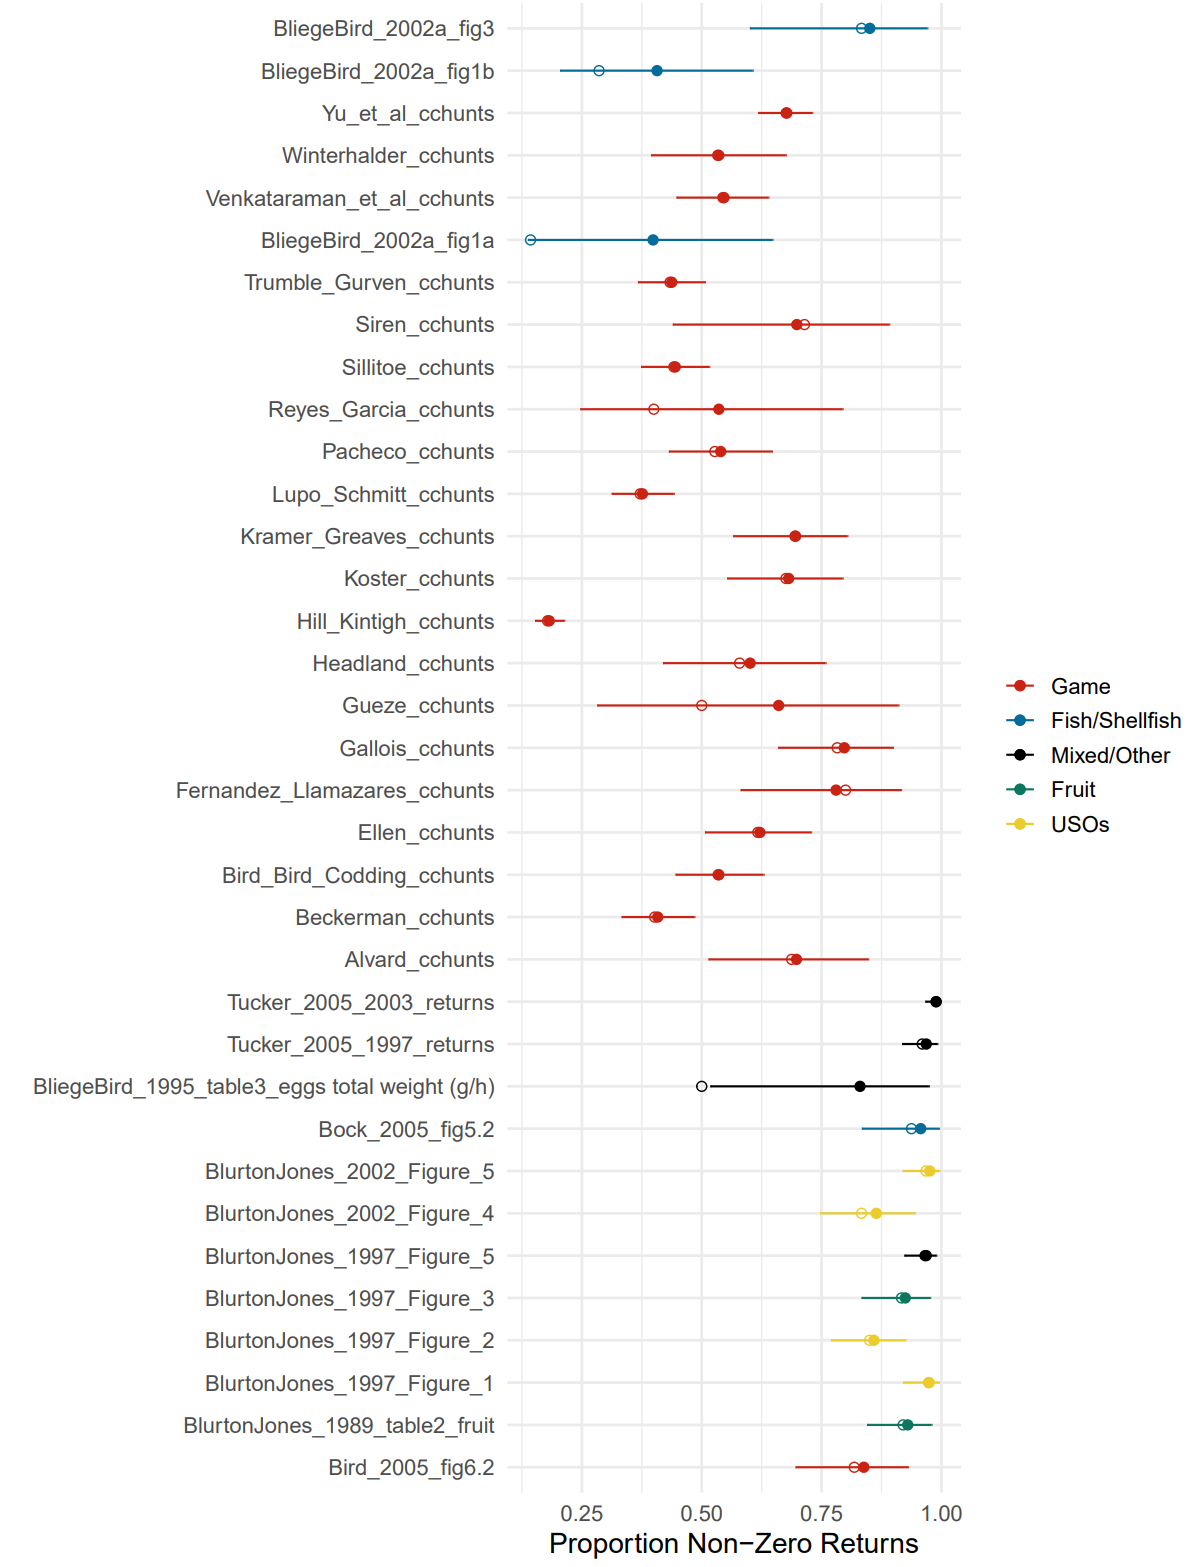
\includegraphics[width=16cm]{text/images/reply_2.png}
        \caption{Probability of zero-returns across outcomes.}
        \label{fig:reply_2}
    \end{figure}
    
    \item "We employed regularizing priors…": Where are these priors reported? \rev{We use bland regularizing priors, in particular  Normal(0,1) for fixed effects (e.g., intercepts), Exponential(1) for the random effect standard deviations and LKJ(2) for the correlations between random effects. We added a section in the supplementary materials with this information.}
    
    \item Page 6, typo: "foraging foraging" \rev{Thanks.}
    
    \item I notice in the github code (very helpful for better understanding what was done here by the  way!) that starting values were fixed to zero for the Stan model (init = "0"). I'm guessing this was done to avoid divergent transitions during estimation with the large number of random effects.  Are there any potential caveats to this approach that should be noted for readers?
    \rev{We've found that with models with many parameters, starting at 0 can be helpful (and in some cases, necessary) for the model to get started sampling. However, after many iterations of warm up there should be no dependence on starting values, unless the model is badly mis-specified or suffers from a multimodal posterior. We used standard MCMC diagnostics and found that all population parameters had Rhat < 1.01 and an effective sample size > 1000. We are thus confident that the model is not influenced by the starting parameters. }
    
    
\end{enumerate}

\section{Reviewer 3}
 
The authors build a large hunter-gatherer dataset of children’s foraging returns from published sources to investigate whether variation in resource complexity drives variation in children’s foraging proficiency. There is much to like about the questions addressed in the manuscript, the work put into constructing the dataset and the complexity of the analysis. Clarifying several points in the set up, methods and analysis would strengthen the argument’s presentation and analytic interpretation.

\subsection{Comments}
\begin{enumerate}
    \item The idea that long childhoods evolved as a protected period for learning complex foraging skills is only one of several competing hypotheses about the evolution of childhood. At least some of the authors elaborate on these alternative propositions in their other work. I would make it clear in the abstract and the first paragraph of the introduction that this is one of several ideas. No need to elaborate, maybe just cite the alternative ideas. As is, it reads as if learning is the only idea on the table. A nod should also be made that variation in foraging returns can occur irrespective of learning \& skill.
    
    \rev{The new introductory paragraphs should provide an answer to this comment.}
    
    \item Related to this, notably, is the absence of a discussion of strength (i.e. Blurton Jones’ argument that age-related variation is about gains in size and strength, not skill). Also see the 2002 Human Nature issue on childhood where the Bock, Blurton Jones, Bliege Bird, Kramer and others address strength vs. skill. This would be important to distinguish because tubers, for example, aren’t so much skill intensive as strength dependent, which varies cross culturally (e.g. Hadza roots are huge, whereas New World tubers can be quite small, and in a sandy substrate, meaning that children of all ages can access, whereas Hadza roots may be less accessible to children). That level of detail is beyond the scope of the article, but it’s still worth discussing where the authors place strength. Is it a dimension of return rate variation that they’re not considering, or is it conceptually bundled into skill?
    
    \rev{In answer to these points we included more discussion on strength and knowledge in both Introduction and Discussion sections, we highlights the presence of variation even within resources and we clarify that, indeed, strength is conceptually bundled into skill. }
    
    \item The results section I found quite confusing and the text didn’t really seem to match the analytic approach as I could glean from Fig 5 and the methods section. The reader has to spend way too much time trying to piece together the text and figures to understand the analysis, which should be more clearly elaborated on in the text. The text on pg 3 (the paragraph before the Results section) and on pg 4 in the section on the Skill intensity of resources read as if the analytic approach is a tautology \# i.e. return rates are used to define skill intensity, which then determines the rate of return. This is not what the author do in the analysis, I believe, but the text is quite confusing. In trying to unravel the analytic protocol from the figures, rather skill appears to be constructed as a latent variable estimated from age, sex and resource type, and these variables are then included in a model to evaluate variation in return rates. Having reread the text numerous times, I am still very uncertain how the analysis proceeded. To help readers, which for this journal will come from many different scientific backgrounds, in the paragraph before the Result section, I would i) clearly state the analytic goal and shape of the statistical model (for example, you have to search the paper for what the outcome variable is) and ii) briefly describe as a series of analytic steps that follow a figure (for example, mapping elasticities seems to be a side step to get to ‘resource type’ as shown in Fig 5). One suggestion is to move Fig 5 up and use for this purpose, modifying appropriately. A lot of work I’m sure when into this analysis, but it gets lost in trying to sort out the analytic steps taken. This is an inherent problem in journals that put the methods after the results, but it’s incumbent on authors to cleverly insert key methods somewhere before or in the results so they can be interpreted without asking readers to have to piece clues together.
    
    \rev{In answer to this comment, as much as to a similar one from Reviewer 2, we included more information on the statistical analysis in the Introduction and Result sections. Moreover, we included the figure for the Direct acyclic graph earlier in the text, as suggested here. Finally, we specify that all model parameters are estimated jointly, not with sequential regressions. The model we present is indeed complex and has several moving parts, and it is difficult to satisfactorily explain it in a succinct fashion outside of the Methods section. We hope that making the code for statistical analysis open for inspection can help clarify the statistical procedure, although we are aware that the complexity of the analysis makes it hard to critically examine the modelling choices. }
    
    \item I was somewhat disappointed that while the analysis points to children being proficient at some resources earlier in life than others, in the concluding statement (pg 6, lns16-25) the authors fall back on the traditional argument that childhood is about learning. To move the discussion beyond what Kaplan et al. posited in 2000 (and really their argument is about motivation, i.e. learning), and to distinguish the authors’ argument, they might frame more firmly in a new hypothesis or interpretation.
    
    \rev{we are sorry to have disappointed Reviewer 3.} %what to answer here?
    
    \item The graphs and figures are complex, nicely executed and suitable for SA. See comment below about Fig 5. 
    
    \rev{We are pleased Reviewer 3 approves of the plots.}
\end{enumerate}
    
\subsection{Some line-by-line comments}
\begin{enumerate}
    \item pg 2 lns53-56: Define proficiency where it is first used it in the intro. The next sentence describes net production and the age at which production exceeds consumption. Make clear whether proficiency is referring to net production, a measure of efficiency, or some other. I understand that the authors might want to be vague here since they’re trying to summarize many different kinds of analyses.
    \rev{We clarified the definition of proficiency as ``age-specific foraging returns" at the end of the Introduction and use it consistently with the same meaning across the paper. If the Editor/Reviewer 3 think it would be best to specify every time ``age-specific foraging returns" instead of foraging proficiency, we can easily comply.  }
    
    \item Thank you for the very important point that most of these studies are focused on hunting. 
    \rev{You are so, so welcome.}
    
    \item pg 3 lns 24-5: “game and tubers exhibit accelerating returns” state until what age, or through childhood, i.e. at some point they have to plateau.
    \rev{Unfortunately we did not extend the model after 20 years of age, so we do not know when they do plateau (and yes, they must certainly do). We refer to Koster, et al. "The life history of human foraging" 2020, for a detailed analysis of plateau and peak ages for hunting. They find peak age in skill to be quite variable cross culturally, clustering around age 30. No similar study exist for tubers, but future research should address this point as well.  }
    
    \item pg 4 lns 26-29: There are several clarifications needed in these sentences. What are low-skill and high-skill foragers? I would avoid this language or kind of typology. Resources may have different skills to appropriate, but most foragers have a broad mix of resource types. Production here seems to be used interchangeably with return rate? Usually these are different concepts, production the numerator. Confusion could be avoided if terms are clarified earlier in the paper. Also would change out the words ‘improvements’ and ‘delayed’, which suggest that there’s some goal, ie. sounds like a teleology, just describe.
    \rev{We are using here skill in the definition used within the model, so skill is 1) resource specific, 2) includes all individual traits that contribute to foraging returns. We try to clarify this in the highlighted result section. }
    \begin{displayquote}
    This suggests that disparities in production between low skill and high skill foragers are more apparent for more complex resource types \textcolor{red}{(with skill defined as the resource specific latent trait measured by our model, which combines the individual characteristics relevant for that type of foraging)}. 
    \end{displayquote}
    \rev{We also take seriously the comments on lexicon, so many papers become hard to read because it's hard to keep track of what the authors mean. So, having defined proficiency in our paper as age-specific returns, we now use this term through the whole paper, instead of moving back and fro through other not-so-fitting words. Concerning the apparent teleology of words like ``improving" and ``delaying" we believe that they do a reasonably good job of describing changes along an axis, that of productivity, that has some implicit ``better" and ``worse" in human behavioral ecology, with the general idea that producing more food is better than producing less. But if the Editor and Reviewer 3 disagree with this view, we are happy to look for less qualitatively charged synonims. }
    
    \item pg 4 lns 30-4: ‘n, the parameter indicating skill intensity’ , later in the paragraph it states ‘n indicates how much foraging returns depend on skill, i.e. how much skill is necessary to obtain a certain amount of returns’ It’s not clear how this is not a tautology where skill defines complexity, and complexity is assumed to structure skill, and there’s no independent measure of skill. Avoid or clarify such language.
    \rev{In our dataset, we defined complexity of the four resource types according to certain characteristics, as defined in the literature. It does not depend on skill as estimated by our model, but rather we are comparing skill intensity and the shape of the curve describing the development of skill for each of these resources. Comparing the four resources we connect the pattern of variation to the complexity of these activities. A quantitative approach to defining resource complexity would be advisable, but again, ethnographic details would be needed to appropriately code complexity. We hope future work will build on both the code and at least part of the dataset provided here and tackle with more detail the definition of resource complexity.    }
    
    \item Also define ‘skill intensity’ when first used. Is it different from ‘foraging skill’ or resource complexity as ‘hard’ or ‘easy’. It reads like age-specific return rates are used to define skill (an underlying latent variable).
    \rev{We appreciate that the model has several complex parts interacting with one another and that we need to improve the way we describe it to the reader. In particular, we definitely need to clarify the difference between skill, a latent variable that describe the variation of individual traits with age, and skill intensity, which is how much skill a certain resource requires for collection. In practical terms, for example, let's say that the only trait necessary to forage both fruit and tubers was strength, and thus define skill as strength. With zero skill, both returns would be zero for both resources. A little bit of skill (strength) would allow an individual to reach a big proportion of maximum returns in fruits, but just a limited improvement in tubers. As skill increases, fruit returns would also get better, but not much, because the majority of the improvement has been reached early on. With tubers, instead, only a large amount of skill can guarantee to achieve high returns. The parameter $\eta$ describes how much skill an activity requires to have high returns. We try to clarify this point by rearranging and specifying the meaning of $\eta$ in the relevant Returns paragraph (shown here).   }
    \begin{displayquote}
    Our statistical analysis separately models the changes in age-specific returns and the underlying latent variable, skill. Skill summarizes the traits that are important for foraging. \textcolor{red}{Figure \ref{fig:eta}, instead, shows the posterior distribution for $\eta$, the parameter indicating skill intensity.} $\eta$ indicates how much foraging returns depend on skill, i.e., how much skill is necessary to obtain a certain amount of returns \textcolor{red}{($\eta$ is the exponent of skill $S$ and regulates its effect on returns, falling on the arrow that connects Skill to Returns in the DAG in [FIGUREXXX])}. The four types of resources analyzed here differ in how skill-intensive they are, with game and tubers requiring more skill, fruit requiring less skill, and fish/shellfish in between (figure \ref{fig:eta}, left). 
    \end{displayquote}
    
    \item pg 4 ln 41: ‘our predictions’, what predictions? It would be useful to state in analytic terms as per previous comments about a paragraph you might insert before the Results section.
    \rev{Prediction here is used in its statistical meaning, to define the predicted differences with sex according to the model, not as a reference to hypotheses to be tested. We hope this satisfies the question of Reviewer 3, but we can also provide mathematical description of the predicted values.  }
    
    \item pg 4 ln 44-45: easy and hard to resources? This is the first time this language is used? What are these? This distinction is defined in the methods, but the authors need to find a way to move some of this critical information up into the set up and results – one of the great handicaps of the methods following the results, but the authors need to find a graceful way to incorporate some of these key concepts and definitions earlier in the manuscript. It’s not generally clear how ‘skill intensity’ and ‘resource complexity’ relate to each other (again a conceptual figure might help to clarify or using consistent language).
    \rev{We used in this paragraph easy vs. hard in lieu of more and less complex, probably inducing confusion. We then modified the text to keep consistent a definition, and also better defined the difference between the two in the Introduction  }
    \begin{displayquote}
    Similarly, the sexes do not differ much when compared within resource type, apart from females showing some more differences in the age specific returns between \textcolor{red}{more complex resources and less complex ones} than males (see figure \ref{fig:females_only} and \ref{fig:males_only}). 
    \end{displayquote}
    \begin{displayquote}
    \textcolor{red}{Complexity of resources has been defined in the literature on the basis of certain characteristics that make them difficult to acquire \citep{schuppli_life_2016, veile_hunter-gatherer_2018}. These include food items embedded a hard substratum, mobile preys, ephemeral/seasonal food products that requires environmental knowledge to be acquired or food products for which specialized technologies are necessary. We hence consider the four resources as differing in complexity, with fruits and marine resources being relatively easier, and game and tubers being harder. }
    \end{displayquote}
    
    \item pg 4 on 46-50: not sure if you need such a strong caveat here for not finding sex differences. I would delete the word ‘presumably’ as there’s no real reason except that it’s traditionally thought boys do the harder stuff.
    \rev{We definitely used an excess of caution here. We removed the `presumably'. }
    \begin{displayquote}
    Instead, it may be that our data is of insufficient resolution to detect differences between male and female foragers--which are \cancel{presumably} smaller than differences between resource types. 
    \end{displayquote}
     
    \item pg 4 ln 52: here’s another place, I would add ‘one theory of childhood” is theorized ...
    \rev{We find this comment in contrast with comment XXX from Reviewer 1, who praised this sentence. We hope that the explanations we provided in the Introduction, plus a small rephrasing here are sufficient to clarify that we do not believe ECT to be the only hypothesis for the evolution of childhood.}
    \begin{displayquote}
    Childhood \textcolor{red}{has been} theorized to have evolved as an extended learning period for collecting complex resources.
    \end{displayquote}
    
    \item pg 6 ln16 and other places throughout. The authors appear to use ‘production and ‘return rate’ interchangeably. I’d be consistent.
    \rev{We thank reviewer 3 for pointing out these inconsistencies in the use of lexicon. As described before, we shifted to `proficiency' through the whole paper. }
    
    \item pg. 7 lns 76-83: it wasn’t clear why resources are additional defined as ‘hard’ or ‘easy’, in what analytic step does this occurs, and does classifying ‘resource complexity’ differ from ‘foraging skill’ shown in Fig 5.
    \rev{We hope to have clarified the definitions of complexity and skill through the paper. We also replaced hard and easy with varying complexity for consistency. }
    \begin{displayquote}
    Resources were defined as \textcolor{red}{more} (game, underground storage organs such as tubers) or \textcolor{red}{less complex} (fruit, fish/shellfish), according to definitions of complexity offered in \citet{johnson_trade-offs_2004}, \citet{lancaster_evolution_2000} and \citet{ schuppli_life_2016}. 
    \end{displayquote}
    
    \item Fig 5, What is ‘return time’ in the caption? Sex is shown to influence foraging returns, but not age. Here’s another place in the text, that reads a bit like an analytic tautology (but I don’t think the analysis actually is, so the authors might take some care that’s it’s not misrepresented as such). Might add that the coefficient n is derived in the analytic step in arrow from ‘foraging skill’ to ‘foraging returns’. I think much could be clarified throughout about the analysis if this figure came earlier in the article, and described in a few sentences before the results, as it seems to be the backbone of the analytic approach.
    \rev{'Resource time' was definitely a typo, should be 'resource type'. Concerning age, instead, our model treats all effects of age as passing through skill (the sum of all age-varying traits that influence returns), apart, of course, the influence that age has on the choice of resource (children begin to perform different activities at varying ages). Finally, Reviewer 3's suggestion to bring the graph showing the DAG earlier in the text, and to explain $\eta$ on the basis of this graph are very welcome are we are happy to comply.}
    \begin{displayquote}
    \textcolor{red}{($\eta$ is the exponent of skill $S$ and regulates its effect on returns, falling on the arrow that connects Skill to Returns in the DAG in \ref{fig:Figure_1.png})}
    \end{displayquote}

\end{enumerate}

\rev{We are especially grateful to Reviewer 3 for the attention to the lexicon we used and the consistency of the vocabulary used. It's so easy to loose the feeling that too many words are used to define the same thing. }


\bibliography{references.bib}

\end{document}